\documentclass[11pt]{article}

\usepackage[a4paper,margin=1in]{geometry}
\usepackage{amsmath,amssymb,amsthm,mathtools}
\usepackage{booktabs}
\usepackage{graphicx}
\usepackage{subcaption}
\usepackage{multirow}
\usepackage{array}
\usepackage[hidelinks,colorlinks=true,linkcolor=blue!50!black,citecolor=blue!50!black,urlcolor=blue!60!black]{hyperref}
\usepackage{enumitem}
\usepackage{setspace}
\usepackage{algorithm}
\usepackage{algpseudocode}
\usepackage{xcolor}
\usepackage{tcolorbox}

\onehalfspacing

% Theorem environments
\newtheorem{theorem}{Theorem}
\newtheorem{proposition}[theorem]{Proposition}
\newtheorem{lemma}[theorem]{Lemma}
\newtheorem{corollary}[theorem]{Corollary}
\theoremstyle{definition}
\newtheorem{definition}[theorem]{Definition}
\newtheorem{assumption}[theorem]{Assumption}
\theoremstyle{remark}
\newtheorem{remark}[theorem]{Remark}

% Notation
\newcommand{\R}{\mathbb{R}}
\newcommand{\PP}{\mathbb{P}}
\newcommand{\EE}{\mathbb{E}}
\newcommand{\Ddata}{\mathcal{D}_{\text{data}}}
\newcommand{\Dfit}{\mathcal{D}_{\text{fit}}}
\newcommand{\Dcal}{\mathcal{D}_{\text{cal}}}
\newcommand{\Dtest}{\mathcal{D}_{\text{test}}}
\newcommand{\sphys}{\sigma_{\mathrm{phys}}}
\newcommand{\TV}{\mathrm{TV}}
\newcommand{\PICP}{\mathrm{PI\text{-}CP}}
\newcommand{\Rop}{\mathcal{R}}
\newcommand{\ind}{\mathbf{1}}

\title{
\textbf{Physics-Informed Conformal Prediction (PI-CP)}\\[0.4em]
\large Distribution-Free Uncertainty Quantification for\\
Physics-Informed Neural Networks with Shock Structures\\[0.6em]
\normalsize\textit{Progress Report}
}


\date{\today}

\begin{document}

\maketitle

\begin{abstract}
\noindent
We introduce Physics-Informed Conformal Prediction (PI-CP), a distribution-free, post-hoc uncertainty quantification (UQ) framework for Physics-Informed Neural Networks (PINNs) solving PDEs whose solutions exhibit sharp localised features such as shocks, fronts, and boundary layers. Existing conformal-prediction methods for PINNs guarantee only \emph{marginal} coverage, which can mask systematic under-coverage inside thin shock layers that carry the bulk of the absolute error. PI-CP closes this gap with three components: a PDE-derived nonconformity scale $\sphys$, a graph-regularised conditional-quantile network $g_\phi$ trained on PDE-intrinsic edge anomalies, and conformal calibration stratified by a residual-and-gradient indicator. We prove finite-sample stratified coverage (Theorem~\ref{thm:strat}) under standard exchangeability assumptions, and a piecewise-constant structure theorem for the quantile network under graph-total-variation regularisation (Theorem~\ref{thm:tv}). On the Burgers benchmark at $\nu = 0.01/\pi$, PI-CP achieves per-stratum coverage within $0.015$ of nominal $0.90$ across two PINN architectures (Vanilla MLP and Fourier-feature), with shock-region intervals $3$--$10\times$ wider than smooth-region intervals --- reflecting the genuine heterogeneity of PINN error without sacrificing validity. The framework is architecture-agnostic and treats the trained PINN as a black box exposing only $u_\theta$ and the PDE residual $\Rop(u_\theta)$.
\end{abstract}

\tableofcontents
\newpage

%=================================================================
\section{Introduction}
\label{sec:intro}

Physics-Informed Neural Networks~\cite{raissi2019pinns,karniadakis2021review} have become a standard tool for solving forward and inverse PDE problems, embedding governing equations directly into the training objective. Despite extensive methodological development --- self-adaptive weighting, gradient enhancement, Fourier features, KAN-based parametrisations, geometry-aware variants --- the vast majority of deployed PINNs remain \emph{deterministic} and do not produce uncertainty estimates of any kind.

This deficiency is consequential. PINNs are increasingly used in scientific computing settings where a single point estimate is inadequate: in inverse problems where multiple parameter configurations explain the data, in multi-physics design where decisions must account for predictive uncertainty, and in regions where the PDE solution itself is poorly resolved by the underlying neural surrogate. The need for principled, computationally tractable, and theoretically defensible uncertainty quantification (UQ) for PINNs is now widely recognised.

Existing UQ approaches for PINNs --- Bayesian PINNs via Hamiltonian Monte Carlo or variational inference, Monte Carlo dropout, deep ensembles, distance-based heuristics --- share two structural limitations. First, they rely on distributional assumptions (Gaussian likelihoods, posterior factorisation) that are typically incorrect when the PDE error is concentrated in thin layers. Second, with the exception of recent conformal approaches~\cite{yu2025cp}, they provide no finite-sample coverage guarantee: the user has no rigorous statement about how often the produced uncertainty bands actually contain the truth.

Conformal prediction~\cite{vovk2005,angelopoulos2022gentle} addresses both limitations simultaneously. It is distribution-free, requires only exchangeability between calibration and test data, and produces prediction intervals with finite-sample coverage guarantees regardless of the underlying model's quality. Yu, Ho, and Wang~\cite{yu2025cp} recently introduced split conformal prediction into the PINN setting, establishing the first systematic distribution-free UQ for PINNs. Their framework wraps heuristic uncertainty estimators (dropout, latent-distance, B-PINNs) with the scaled nonconformity score and recovers marginal coverage guarantees.

\paragraph{The marginal-coverage gap.} The guarantee in~\cite{yu2025cp} is \emph{marginal}: coverage is averaged over the entire spatio-temporal domain. For PDEs with sharp localised features --- viscous Burgers at small $\nu$, Allen--Cahn near interfaces, Navier--Stokes within boundary layers --- this average masks structural under-coverage. The PINN's pointwise error is concentrated in a layer of small Lebesgue measure but large amplitude. A method achieving $90\%$ marginal coverage can deliver $70\%$ coverage \emph{inside} the layer while delivering $95\%$ \emph{outside}. The user cares about the layer, but the guarantee does not.

\paragraph{Our contribution.} We propose Physics-Informed Conformal Prediction (PI-CP), a post-hoc UQ framework that
\begin{enumerate}[leftmargin=*,topsep=2pt,itemsep=2pt]
    \item provides finite-sample distribution-free coverage \emph{conditional on a PDE-derived stratification} of the spatio-temporal domain (Theorem~\ref{thm:strat});
    \item adapts interval widths to local PDE difficulty via a physics-informed scale $\sphys$ and a conditional-quantile network $g_\phi$;
    \item incorporates PDE-intrinsic graph regularisation that yields approximately piecewise-constant uncertainty structure (Theorem~\ref{thm:tv}); and
    \item remains \emph{architecture-agnostic}: the framework wraps any trained PINN exposing only $u_\theta(x)$ and the PDE residual $\Rop(u_\theta)(x)$.
\end{enumerate}

The framework treats the PINN as a black box and does not modify training. The contribution lies entirely on the UQ side rather than the approximation side, which we emphasise to clearly delineate scope: PI-CP does not improve the PINN's point predictions, but it produces calibrated uncertainty around them.

\paragraph{Organisation.} Section~\ref{sec:rw} reviews related work. Section~\ref{sec:setting} fixes notation and the formal setting. Section~\ref{sec:method} develops the three PI-CP components. Section~\ref{sec:theory} states and proves the two main theorems. Section~\ref{sec:algorithm} presents the complete algorithm. Section~\ref{sec:experiments} reports empirical results on the Burgers benchmark across two PINN architectures. Section~\ref{sec:limitations} discusses honest scoping. Section~\ref{sec:future} outlines remaining work.

%=================================================================
\section{Related Work}
\label{sec:rw}

\paragraph{Conformal prediction.} Conformal prediction was introduced by Vovk, Gammerman and Saunders~\cite{vovk2005} and has since been developed into a comprehensive distribution-free UQ framework~\cite{angelopoulos2022gentle}. The core split-CP procedure constructs prediction intervals by computing nonconformity scores on a held-out calibration set and using their empirical quantile as a threshold. Key extensions include conformalised quantile regression~\cite{romano2019cqr}, class-conditional CP, weighted CP for covariate shift~\cite{tibshirani2019weighted}, and conformal risk control~\cite{angelopoulos2022crisk}. We build directly on the class-conditional construction and on the scaled-score formulation of~\cite{romano2019cqr}.

\paragraph{Conformal prediction for scientific machine learning.} Beyond~\cite{yu2025cp}, recent work has applied conformal methods to deep operator networks~\cite{moya2024deeponet}, Kolmogorov--Arnold networks~\cite{moya2025kan}, interatomic potentials~\cite{hu2022conformal}, and surrogate models for spatio-temporal systems~\cite{gopakumar2024surrogate}. None of these address PDE-derived stratification or shock-bearing systems specifically.

\paragraph{Uncertainty quantification for PINNs.} B-PINNs~\cite{yang2021bpinns} provide a Bayesian formulation via HMC or VI. Monte Carlo dropout~\cite{gal2016dropout} offers a cheap variational approximation. Ensembles aggregate independent runs. All these are surveyed comprehensively in~\cite{yu2025cp}. None provide distribution-free finite-sample guarantees, and all suffer in shock regions due to Gaussian or unimodal posterior assumptions.

\paragraph{Distinction from prior work.} PI-CP differs from~\cite{yu2025cp} in three ways. First, our guarantee is stratified rather than marginal: it holds \emph{within} each PDE-difficulty regime. Second, the stratification map is derived from PDE quantities ($|\Rop(u_\theta)|$ and $\|\nabla u_\theta\|$), making it intrinsic to the problem rather than feature-based. Third, the conditional-quantile network is regularised by a graph-total-variation penalty on PDE-intrinsic edge weights, which provides an inductive bias matching the piecewise-smooth structure of shock-bearing PDE solutions --- a smooth MLP cannot achieve this.

%=================================================================
\section{Problem Setting and Notation}
\label{sec:setting}

\subsection{The PDE and PINN}

Let $\Omega \subset \R^d$ be a bounded spatial domain and $T > 0$ a terminal time. Consider the initial-boundary value problem
\begin{align}
    \mathcal{L}[u](x,t) &= f(x,t), \quad (x,t) \in \Omega \times (0,T], \label{eq:pde}\\
    u(x,0) &= u_0(x), \quad x \in \Omega, \\
    \mathcal{B}[u](x,t) &= g(x,t), \quad (x,t) \in \partial\Omega \times (0,T],
\end{align}
where $\mathcal{L}$ is a (possibly nonlinear) differential operator and $\mathcal{B}$ encodes boundary conditions. A PINN approximates $u$ by a neural network $u_\theta: \Omega \times [0,T] \to \R$ trained to minimise a composite loss combining data fidelity, PDE residual, and initial/boundary penalties. The pointwise residual is
\begin{equation}
    \Rop(u_\theta)(x,t) := \mathcal{L}[u_\theta](x,t) - f(x,t).
    \label{eq:residual}
\end{equation}

For Burgers' equation $u_t + uu_x - \nu u_{xx} = 0$, which is our primary benchmark, $\Rop(u_\theta) = \partial_t u_\theta + u_\theta\, \partial_x u_\theta - \nu\, \partial_{xx} u_\theta$.

\subsection{Data and folds}

We require labelled data $\{(X_i, U_i)\}_{i=1}^N$ drawn i.i.d.\ from a Borel measure $\PP$ on $\mathcal{X} \times \R$, where $\mathcal{X} = \Omega \times [0,T]$. We partition the indices into four mutually disjoint folds:
\begin{equation}
    \{1,\dots,N\} = \mathcal{I}_{\text{data}} \sqcup \mathcal{I}_{\text{fit}} \sqcup \mathcal{I}_{\text{cal}} \sqcup \mathcal{I}_{\text{test}},
\end{equation}
with corresponding data subsets $\Ddata, \Dfit, \Dcal, \Dtest$. The PINN $u_\theta$ is trained on $\Ddata$; the conditional-quantile network $g_\phi$ is fit on $\Dfit$; conformal calibration uses $\Dcal$; evaluation uses $\Dtest$. This four-way separation, rather than the conventional three-way (train/cal/test), is required to preserve the measurability hypotheses of Theorem~\ref{thm:strat}.

\subsection{Notation table}

For reference, Table~\ref{tab:notation} summarises notation.

\begin{table}[h]
\centering
\caption{Notation used throughout. Quantities marked $\Ddata$-measurable are computed using only the PINN-training fold.}
\label{tab:notation}
\small
\begin{tabular}{lll}
\toprule
Symbol & Meaning & Domain / Type \\
\midrule
$x = (x_{\text{sp}}, t)$ & Spatio-temporal coordinate & $\mathcal{X} \subset \R^{d+1}$ \\
$u_\theta(x)$ & Trained PINN prediction & $\R$; $\Ddata$-measurable \\
$\Rop(u_\theta)(x)$ & PDE residual & $\R$ \\
$\nabla u_\theta(x)$ & Spatial-temporal gradient & $\R^{d+1}$ \\
$\sphys(x)$ & Physics-informed scale & $\R_{>0}$; $\Ddata$-measurable \\
$g_\phi(x)$ & Conditional-quantile network & $\R_{>0}$; $\Dfit$-measurable \\
$G(x) \in \{0,1\}$ & Stratification indicator & $\{0=\text{smooth}, 1=\text{shock}\}$ \\
$\tau$ & Stratification threshold & $\R_{>0}$; $\Ddata$-measurable \\
$\hat{q}^{(g)}$ & Conformal quantile, stratum $g$ & $\R_{>0}$ \\
$\alpha$ & Miscoverage level & $(0,1)$, target $1{-}\alpha$ \\
$N^{(g)}$ & Calibration-set size in stratum $g$ & $\mathbb{N}$ \\
$\mathcal{C}^{\PICP}_{1-\alpha}(x)$ & PI-CP prediction interval at $x$ & Closed interval $\subset \R$ \\
\bottomrule
\end{tabular}
\end{table}

%=================================================================
\section{The PI-CP Framework}
\label{sec:method}

PI-CP consists of three components applied after the PINN $u_\theta$ has been trained on $\Ddata$. We describe each in turn.

\subsection{Physics-informed scale}
\label{sec:sphys}

Define the physics-informed scale
\begin{equation}
    \sphys(x) := \varepsilon + \beta_1\, |\Rop(u_\theta)(x)|^p + \beta_2\, \|\nabla u_\theta(x)\|^q,
    \label{eq:sphys}
\end{equation}
with floor $\varepsilon > 0$, weights $\beta_1, \beta_2 \geq 0$, and exponents $p, q \in (0, 1]$. In our experiments we use $p = q = 1$ and $\beta_1 = 0$ (gradient-only), giving $\sphys(x) = \varepsilon + \beta_2 \|\nabla u_\theta(x)\|$. The residual term is available for problems where it provides additional sharpness signal; we keep the general form for future extensibility.

The role of $\sphys$ is to act as a \emph{model-side} estimate of local error magnitude. Near a Burgers shock, both $|\Rop(u_\theta)|$ and $\|\nabla u_\theta\|$ scale as $O(\nu^{-1/2})$, so $\sphys$ self-adapts to the shock geometry without any auxiliary training. The nonconformity scores
\begin{equation}
    s_i := \frac{|U_i - u_\theta(X_i)|}{\sphys(X_i)}
    \label{eq:score}
\end{equation}
are dimensionless residuals normalised by this scale; exchangeability of $\{s_i\}$ on $\Dcal$ (preserved because $\sphys$ is $\Ddata$-measurable) is what powers the conformal guarantee.

\subsection{Conditional-quantile network with graph regularisation}
\label{sec:gphi}

We learn a conditional-quantile network $g_\phi : \mathcal{X} \to \R_{>0}$ that estimates the local $(1{-}\alpha)$-quantile of the scaled residual $s$. To inject PDE-intrinsic structure, we build a $k$-NN graph $G_{\text{NN}} = (V, E)$ over the points in $\Dfit$ with edge weights
\begin{equation}
    w_{ij} := \exp\!\left(-\gamma_1 \|X_i - X_j\|^2 - \gamma_2\, \eta_{ij}\right),
    \quad
    \eta_{ij} := |\Rop(u_\theta)(X_i) - \Rop(u_\theta)(X_j)| + \kappa |u_\theta(X_i) - u_\theta(X_j)|.
    \label{eq:edge}
\end{equation}
The edge anomaly $\eta_{ij}$ is small in PDE-smooth regions (both residuals and solution values vary slowly) and large across shock fronts (where residual and solution jumps are correlated and large). The edge weight $w_{ij}$ inversely reflects this: edges across shocks have small weight.

We fit $g_\phi$ on $\Dfit$ by minimising the graph-TV-regularised pinball loss
\begin{equation}
    \mathcal{F}(\phi) :=
    \underbrace{\frac{1}{|\Dfit|}\sum_{i \in \mathcal{I}_{\text{fit}}} \rho_{1-\alpha}\!\big(s_i - g_\phi(X_i)\big)}_{\text{pinball data fit}}
    \;+\; \lambda_{\TV}\!\!\!\!\sum_{(i,j)\in E}\!\!\!\! w_{ij}\,|g_\phi(X_i) - g_\phi(X_j)|
    \;+\; \tfrac{\mu}{2} \|g_\phi\|_2^2,
    \label{eq:gphi-loss}
\end{equation}
where $\rho_{1-\alpha}(r) = (1{-}\alpha)\, r_+ + \alpha\, (-r)_+$ is the pinball loss at quantile level $1{-}\alpha$, and $\mu > 0$ adds strong convexity. The TV term penalises differences across edges of high weight (smooth-region edges) and is permissive across low-weight edges (shock-front edges), encouraging $g_\phi$ to be approximately piecewise constant on PDE-smooth regions while permitting jumps across shocks. Theorem~\ref{thm:tv} formalises this.

\subsection{Shock-stratified conformal calibration}
\label{sec:stratify}

Define the shock indicator
\begin{equation}
    G(x) := \ind\big\{|\Rop(u_\theta)(x)| + \kappa\,\|\nabla u_\theta(x)\| > \tau\big\} \in \{0, 1\},
    \label{eq:strat}
\end{equation}
with threshold $\tau$ taken as the $90$th percentile of the indicator $|\Rop(u_\theta)(\cdot)| + \kappa\|\nabla u_\theta(\cdot)\|$ \emph{on the training fold $\Ddata$}. Both $\tau$ and $G$ are thus $\Ddata$-measurable, a property essential for Theorem~\ref{thm:strat}.

For each stratum $g \in \{0, 1\}$, compute the in-stratum scaled scores on $\Dcal$:
\begin{equation}
    \ell_j := \frac{|U_j - u_\theta(X_j)|}{\sphys(X_j) \cdot g_\phi(X_j)},
    \quad j \in \mathcal{I}_{\text{cal}},\; G(X_j) = g,
    \label{eq:loc-score}
\end{equation}
and define the conformal quantile
\begin{equation}
    \hat{q}^{(g)} := \ell^{(g)}_{(k(g))},
    \quad
    k(g) = \lceil (N^{(g)} + 1)(1 - \alpha) \rceil,
    \label{eq:qhat}
\end{equation}
where $\ell^{(g)}_{(1)} \leq \dots \leq \ell^{(g)}_{(N^{(g)})}$ are the order statistics of the stratum-$g$ calibration scores. When $N^{(g)} < \lceil 1/\alpha \rceil - 1$ we set $\hat{q}^{(g)} = +\infty$, yielding the trivial interval; this preserves coverage validity at the cost of informativeness for severely under-represented strata.

The PI-CP prediction interval at a test point $x_{\text{new}}$ is
\begin{equation}
    \mathcal{C}^{\PICP}_{1-\alpha}(x_{\text{new}}) := \Big[ u_\theta(x_{\text{new}}) \pm \hat{q}^{(G(x_{\text{new}}))} \cdot g_\phi(x_{\text{new}}) \cdot \sphys(x_{\text{new}}) \Big].
    \label{eq:interval}
\end{equation}

%=================================================================
\section{Theoretical Guarantees}
\label{sec:theory}

\subsection{Stratified finite-sample coverage}

\begin{assumption}[Exchangeability and measurability]
\label{ass:main}
The data $\{(X_i, U_i)\}_{i \in \mathcal{I}_{\text{data}} \cup \mathcal{I}_{\text{fit}} \cup \mathcal{I}_{\text{cal}}}$ together with $(X_{\text{new}}, U_{\text{new}})$ are i.i.d.\ from a Borel measure $\PP$ on $\mathcal{X} \times \R$. The functions $u_\theta$, $\sphys$, $g_\phi$, and $G$ are measurable with respect to $\sigma(\Ddata \cup \Dfit)$, and in particular do not depend on $\Dcal$ or $(X_{\text{new}}, U_{\text{new}})$.
\end{assumption}

\begin{theorem}[Stratified finite-sample coverage]
\label{thm:strat}
Under Assumption~\ref{ass:main}, for every $\alpha \in (0,1)$ and every $g \in \{0, 1\}$ with $\PP(G(X) = g) > 0$,
\begin{equation}
    \PP\!\left( U_{\text{new}} \in \mathcal{C}^{\PICP}_{1-\alpha}(X_{\text{new}}) \;\middle|\; G(X_{\text{new}}) = g \right) \;\geq\; 1 - \alpha.
    \label{eq:strat-cov}
\end{equation}
If the conditional law of the scaled score $\ell_{\text{new}}$ given $G(X_{\text{new}}) = g$ is atomless, the bound is sharp up to a finite-sample correction:
\begin{equation}
    \PP\!\left( U_{\text{new}} \in \mathcal{C}^{\PICP}_{1-\alpha}(X_{\text{new}}) \;\middle|\; G(X_{\text{new}}) = g \right) \;\leq\; 1 - \alpha + \EE\!\left[\tfrac{1}{N^{(g)} + 1} \;\middle|\; G(X_{\text{new}}) = g\right].
\end{equation}
\end{theorem}

\begin{proof}
We condition on $\sigma(\Ddata \cup \Dfit)$ throughout, so that $u_\theta$, $\sphys$, $g_\phi$, $G$, and $\tau$ are all deterministic functions. Fix $g$ with $\PP(G(X) = g) > 0$. Let $\mathcal{J}^{(g)} \subseteq \mathcal{I}_{\text{cal}}$ be the random subset of calibration indices satisfying $G(X_j) = g$, with realised size $N^{(g)}$.

\textbf{Step 1 (within-stratum conditional i.i.d.).} Conditional on $\sigma(\Ddata \cup \Dfit) \cup \{G(X_j)\}_{j \in \mathcal{I}_{\text{cal}}} \cup \{G(X_{\text{new}}) = g\}$, the calibration pairs $\{(X_j, U_j)\}_{j \in \mathcal{J}^{(g)}}$ together with $(X_{\text{new}}, U_{\text{new}})$ are mutually independent, each with conditional law $\PP(\cdot \mid G(X) = g)$. This follows because the original pairs are i.i.d., $G$ is a measurable function of $X$ only, and conditioning on the values of $G$ at the calibration points and the test point acts independently on each pair.

\textbf{Step 2 (exchangeability of scaled scores).} The scaled scores $\ell_j = |U_j - u_\theta(X_j)|/(\sphys(X_j)\, g_\phi(X_j))$ for $j \in \mathcal{J}^{(g)} \cup \{\text{new}\}$ are deterministic functions of the conditionally i.i.d.\ pairs of Step~1, hence themselves conditionally i.i.d.\ and therefore exchangeable.

\textbf{Step 3 (rank argument).} By exchangeability, the rank of $\ell_{\text{new}}$ among $\{\ell_j\}_{j \in \mathcal{J}^{(g)}} \cup \{\ell_{\text{new}}\}$ is uniform on $\{1, \dots, N^{(g)} + 1\}$. Setting $k = k(g) = \lceil (N^{(g)} + 1)(1 - \alpha) \rceil$,
\begin{equation}
    \PP\big(\ell_{\text{new}} \leq \ell_{(k)} \,\big|\, \text{conditioning}\big) \;\geq\; \frac{k}{N^{(g)} + 1} \;\geq\; 1 - \alpha,
\end{equation}
with equality (up to the discretisation $1/(N^{(g)}+1)$) under continuity. The event $\{\ell_{\text{new}} \leq \ell_{(k)}\}$ is identical to $\{U_{\text{new}} \in \mathcal{C}^{\PICP}_{1-\alpha}(X_{\text{new}})\}$ by definition of the interval~\eqref{eq:interval} and the symmetry of $|\cdot|$.

\textbf{Step 4 (marginalisation).} Taking expectations over $\sigma(\Ddata \cup \Dfit)$ and the stratum labels of the other calibration points (with $G(X_{\text{new}}) = g$ held fixed) yields the stated bound by the tower property. The case $N^{(g)} < \lceil 1/\alpha \rceil - 1$ gives $\hat{q}^{(g)} = +\infty$ and the bound holds trivially.
\end{proof}

\begin{remark}[Comparison to prior work]
When $G$ is constant (single stratum), Theorem~\ref{thm:strat} reduces to Theorem~5.1 of~\cite{yu2025cp} --- the marginal coverage of Local CP. When $G$ is derived from a categorical input feature and $\sphys, g_\phi$ are trivial, it specialises to the class-conditional CP of~\cite[\S4.2]{angelopoulos2022gentle}. The novelty is that $G$ is \emph{PDE-derived} (a function of $u_\theta$, $\Rop(u_\theta)$, and $\tau$), which is permissible because all three are $\Ddata$-measurable.
\end{remark}

\begin{corollary}[Architecture invariance]
\label{cor:arch}
Theorem~\ref{thm:strat} holds for any measurable training procedure producing $u_\theta$ from $\Ddata$. The bound does not depend on the PINN architecture (Vanilla, Fourier-feature, SA-PINN, gPINN, or others), the activation function, or the training algorithm.
\end{corollary}
\subsection{Graph-TV piecewise-constant structure}

The second theorem describes the structure imposed on $g_\phi$ by the graph-TV regulariser. For exposition we state the single-edge form; the component-wise version is technically heavier and is deferred.

\begin{theorem}[Single-edge piecewise-constant structure]
\label{thm:tv}
Let $\mathbf{g}^\star = (g^\star_1, \dots, g^\star_N)$ be the unique minimiser of the discrete graph-TV pinball objective (the node-value version of~\eqref{eq:gphi-loss}, $\mu > 0$). For an edge $(i, j) \in E$, define
\[
    D_{ij} := \sup\{|p_i - p_j| : p_\ell \in \partial \rho_{1-\alpha}(s_\ell - g^\star_\ell),\; \ell \in \{i,j\}\},
    \qquad
    W^{\text{out}}_{ij} := \!\!\!\sum_{\substack{k:(i,k)\in E \\ k \neq j}}\!\!\! w_{ik} + \!\!\!\sum_{\substack{k:(j,k)\in E \\ k \neq i}}\!\!\! w_{jk}.
\]
If
\begin{equation}
    2\lambda_{\TV} w_{ij} \;\geq\; D_{ij} + \lambda_{\TV} W^{\text{out}}_{ij} + \mu (|g^\star_i| + |g^\star_j|),
    \tag{$\dagger$}\label{eq:dag}
\end{equation}
then $g^\star_i = g^\star_j$. In general,
\begin{equation}
    |g^\star_i - g^\star_j| \;\leq\; \frac{1}{\mu}\Big[ D_{ij} + \lambda_{\TV} W^{\text{out}}_{ij} - 2\lambda_{\TV} w_{ij} \Big]_+.
\end{equation}
\end{theorem}

\begin{proof}[Proof sketch]
The objective is strongly convex (via the $\mu$-ridge), so the minimiser is unique. The KKT conditions at nodes $i$ and $j$ involve subgradients of the pinball loss, subgradients of $|g_i - g_j|$ (the absolute value), and the ridge gradient. Subtracting the two KKT equations and isolating the edge $(i, j)$'s contribution via complementary slackness $z^\star_{(i,j)} = w_{ij} \operatorname{sgn}(g^\star_i - g^\star_j)$ when $g^\star_i \neq g^\star_j$ gives the displayed bound. The strict inequality~\eqref{eq:dag} yields a contradiction with $g^\star_i \neq g^\star_j$, hence equality.
\end{proof}

\begin{remark}[PDE-intrinsic interpretation]
Substituting the edge weight~\eqref{eq:edge} into~\eqref{eq:dag} and solving for $\eta_{ij}$ gives that the flatness condition holds whenever
\begin{equation}
    \eta_{ij} \leq \frac{1}{\gamma_2} \log\frac{2\lambda_{\TV}\, e^{-\gamma_1 \|X_i - X_j\|^2}}{D_{ij} + \lambda_{\TV} W^{\text{out}}_{ij} + \mu(|g^\star_i| + |g^\star_j|)}.
\end{equation}
Edges with small PDE-residual jump and small solution jump (smooth-region edges) are flat; edges across shock fronts are permitted to carry jumps. This is the right inductive bias for shock PDEs and is impossible for a coordinate MLP $g_\phi$, whose continuous-function class cannot represent the jump.
\end{remark}

\begin{remark}[Validity is decoupled from regularisation]
Theorem~\ref{thm:strat} does not depend on Theorem~\ref{thm:tv}: coverage validity holds for \emph{any} measurable choice of $g_\phi$ (including $g_\phi \equiv 1$), regardless of the regulariser. The TV penalty affects the \emph{sharpness} of intervals, not their validity. This separation of concerns is desirable: a poorly tuned $\lambda_{\TV}$ produces wider intervals but never invalidates the coverage guarantee.
\end{remark}

%=================================================================
\section{Algorithm}
\label{sec:algorithm}

The complete PI-CP procedure is given in Algorithm~\ref{alg:picp}. The PINN $u_\theta$ is assumed pre-trained on $\Ddata$ using any standard PINN training pipeline. The four-way split $\Ddata, \Dfit, \Dcal, \Dtest$ is i.i.d.\ disjoint.

\begin{algorithm}[t]
\caption{Physics-Informed Conformal Prediction (PI-CP)}
\label{alg:picp}
\begin{algorithmic}[1]
\Require Trained PINN $u_\theta$; folds $\Ddata, \Dfit, \Dcal$; test point $x_{\text{new}}$; level $\alpha$; hyperparameters $(\beta_1, \beta_2, \kappa, \gamma_1, \gamma_2, \lambda_{\TV}, \mu, k_{\text{NN}})$.
\Ensure Prediction interval $\mathcal{C}^{\PICP}_{1-\alpha}(x_{\text{new}})$.
\Statex
\State \textbf{Compute diagnostics} on $\Ddata$: $\Rop(u_\theta)$, $\nabla u_\theta$, $u_\theta$ at each $X_i$.
\State \textbf{Set stratification threshold} $\tau = \text{Quantile}_{0.90}\big(\{|\Rop(u_\theta)(X_i)| + \kappa\|\nabla u_\theta(X_i)\|\}_{i \in \mathcal{I}_{\text{data}}}\big)$.
\State \textbf{Compute scale} $\sphys$ via~\eqref{eq:sphys} on $\Dfit \cup \Dcal \cup \{x_{\text{new}}\}$.
\State \textbf{Compute scores} $s_i = |U_i - u_\theta(X_i)|/\sphys(X_i)$ for $i \in \mathcal{I}_{\text{fit}}$.
\State \textbf{Build $k$-NN graph} on $\Dfit$ with edge weights $w_{ij}$ via~\eqref{eq:edge}.
\State \textbf{Train $g_\phi$} on $\Dfit$ by minimising~\eqref{eq:gphi-loss}.
\State \textbf{Compute strata} $G(X_j)$ for $j \in \mathcal{I}_{\text{cal}}$ via~\eqref{eq:strat}.
\For{$g \in \{0, 1\}$}
    \State Collect $\{\ell_j\}_{j \in \mathcal{I}_{\text{cal}}, G(X_j) = g}$ via~\eqref{eq:loc-score}.
    \State $N^{(g)} \gets |\{j : G(X_j) = g\}|$; \quad $k(g) \gets \lceil (N^{(g)} + 1)(1-\alpha) \rceil$.
    \State $\hat{q}^{(g)} \gets \ell^{(g)}_{(k(g))}$ if $N^{(g)} \geq \lceil 1/\alpha \rceil - 1$, else $+\infty$.
\EndFor
\State \textbf{Predict.} Compute $G(x_{\text{new}})$, $\sphys(x_{\text{new}})$, $g_\phi(x_{\text{new}})$.
\State \Return $\big[u_\theta(x_{\text{new}}) \pm \hat{q}^{(G(x_{\text{new}}))} \cdot g_\phi(x_{\text{new}}) \cdot \sphys(x_{\text{new}})\big]$.
\end{algorithmic}
\end{algorithm}

The computational cost is dominated by (i) the PINN forward+gradient passes on each fold (linear in fold size), (ii) the $k$-NN graph construction ($O(N \log N)$ with KD-trees), and (iii) the $g_\phi$ training ($O(\text{epochs} \times (|\Dfit| + |E|))$). All steps are embarrassingly parallel across architectures, allowing direct re-use of the framework for multiple PINN variants.

%=================================================================
\section{Experiments}
\label{sec:experiments}

\subsection{Benchmark and setup}

\paragraph{PDE.} Viscous Burgers' equation
\begin{equation}
    u_t + u u_x - \nu u_{xx} = 0,
    \quad
    \nu = \frac{0.01}{\pi},
    \quad
    (x, t) \in [-1, 1] \times [0, 1],
\end{equation}
with initial condition $u(x, 0) = -\sin(\pi x)$ and Dirichlet boundaries $u(\pm 1, t) = 0$. The reference solution is the standard Raissi--Karniadakis dataset on a $256 \times 100$ grid ($25\,600$ points).

\paragraph{Splits.} Four mutually disjoint i.i.d.\ folds: $|\Ddata| = 5\,120$ ($20\%$), $|\Dfit| = 3\,840$ ($15\%$), $|\Dcal| = 6\,400$ ($25\%$), $|\Dtest| = 10\,240$ ($40\%$).

\paragraph{PINN architectures.} Two are evaluated: a Vanilla MLP (five hidden layers, width $64$, $\tanh$) and a Fourier-feature MLP (random feature dimension $20$, width $64$). Both are trained with $8\,000$ Adam epochs followed by $1\,500$ L-BFGS iterations with strong Wolfe line search. The L-BFGS phase is essential for resolving the shock; Adam-only training stalls at $L^2$-relative error $\sim 10^{-2}$ whereas the combined schedule achieves $\sim 10^{-3}$ (Vanilla) and $\sim 10^{-4}$ (Fourier).

\paragraph{PI-CP hyperparameters.} $\alpha = 0.10$; $\beta_2 = 0.5$, $\varepsilon = 10^{-3}$ in $\sphys$; $k_{\text{NN}} = 10$; $\gamma_1 = 5$, $\gamma_2 = 2$; $\lambda_{\TV} = 0.05$; $\mu = 0.01$; $\kappa = 0.5$. The stratification threshold $\tau$ is the $90$th percentile of the indicator on $\Ddata$, giving a target shock-stratum mass of $\approx 10\%$.

\subsection{Diagnostic figures}

\paragraph{Stratification (Figure~\ref{fig:strat}).} The PDE-derived indicator $|\Rop(u_\theta)| + \kappa\|\nabla u_\theta\|$ thresholded at the $90$th training-fold percentile correctly identifies the shock structure of Burgers' equation: a thin diagonal band emanating from $(x, t) = (\pm 0.25, 0)$ and converging at $(0, 1)$, with the characteristic triangular fan shape. The stratification is consistent across both architectures, with stratum sizes (test fold): Vanilla $905/10\,240 \approx 8.8\%$, Fourier $906/10\,240 \approx 8.8\%$ --- matching the design target of $\approx 10\%$. The small clusters of shock-flagged points near $x = \pm 1, t \approx 0$ reflect initial-boundary corner effects rather than a shock proper, but are harmless: the conformal validity holds within whatever stratification the indicator produces.

\begin{figure}[t]
\centering
\begin{subfigure}[t]{0.98\textwidth}
    \centering
    \includegraphics[width=\linewidth]{figures/fig1_stratification_Vanilla.png}
    \caption{Vanilla PINN. Shock stratum: $905$ points ($8.84\%$).}
\end{subfigure}
\\[0.4em]
\begin{subfigure}[t]{0.98\textwidth}
    \centering
    \includegraphics[width=\linewidth]{figures/fig1_stratification_Fourier.png}
    \caption{Fourier-feature PINN. Shock stratum: $906$ points ($8.85\%$).}
\end{subfigure}
\caption{\textbf{PDE-derived stratification on the test fold} for both architectures. The shock stratum (red) traces the characteristic Burgers fan terminating at $(0, 1)$; the smooth stratum (blue) occupies the bulk of the domain. The two architectures produce visually indistinguishable stratifications, confirming that the indicator $|\Rop(u_\theta)| + \kappa\|\nabla u_\theta\|$ is a property of the resolved shock rather than of the architecture used to resolve it.}
\label{fig:strat}
\end{figure}

\paragraph{Score distributions (Figure~\ref{fig:scores}).} The histograms of absolute residual $|U - u_\theta|$ on the test fold, separated by stratum, show the heterogeneity that motivates PI-CP. The smooth-stratum residuals are tightly concentrated near zero; the shock-stratum residuals exhibit a heavy right tail extending to $\sim 0.018$ (Vanilla) and $\sim 0.004$ (Fourier). The two distributions overlap substantially in the bulk near zero, which is expected: not every point in the shock stratum is in fact at the shock location, and stratification on $|\Rop|+\kappa\|\nabla u\|$ is an over-inclusive proxy. The key qualitative observation is that the right tail is shock-only, and this tail is what drives the per-stratum conformal quantile $\hat{q}^{(1)}$ to be much larger than $\hat{q}^{(0)}$.

\begin{figure}[t]
\centering
\begin{subfigure}[t]{0.98\textwidth}
    \centering
    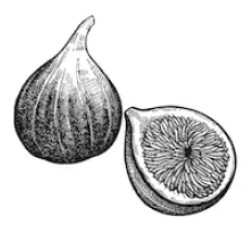
\includegraphics[width=\linewidth]{figures/fig1.png}
    \caption{Vanilla PINN. Smooth residuals concentrate below $5 \times 10^{-4}$; shock residuals extend an order of magnitude further.}
\end{subfigure}
\\[0.4em]
\begin{subfigure}[t]{0.98\textwidth}
    \centering
    \includegraphics[width=\linewidth]{figures/fig2_scores_Fourier.png}
    \caption{Fourier-feature PINN. Smaller scale overall (note axis), but the smooth/shock separation persists.}
\end{subfigure}
\caption{\textbf{Absolute residual distributions per stratum} on the test fold. The right-tail asymmetry in the shock stratum justifies stratified calibration: a single global quantile would either undercover the shock tail or wastefully widen smooth-region intervals.}
\label{fig:scores}
\end{figure}

\paragraph{Residual normality (Figure~\ref{fig:qq}).} The QQ-plots of signed residuals $U - u_\theta$ against a fitted Gaussian show severe non-normality in both strata of both architectures. The smooth stratum exhibits an S-curve characteristic of light-bodied heavy-tailed distributions; the shock stratum shows a sharp asymmetric inflection consistent with a spike-and-slab mixture. Critically, this is the empirical justification for distribution-free UQ: any procedure assuming Gaussian residuals (Bayesian PINN with Gaussian likelihood, MC-dropout treated as posterior variance) would mis-specify the interval shape in exactly the regime where calibration matters most.

\begin{figure}[t]
\centering
\begin{subfigure}[t]{0.98\textwidth}
    \centering
    \includegraphics[width=\linewidth]{figures/fig3_qq_Vanilla.png}
    \caption{Vanilla PINN: smooth stratum (left) shows S-curve heavy tails; shock stratum (right) shows asymmetric heavy left tail.}
\end{subfigure}
\\[0.4em]
\begin{subfigure}[t]{0.98\textwidth}
    \centering
    \includegraphics[width=\linewidth]{figures/fig3_qq_Fourier.png}
    \caption{Fourier-feature PINN: less pronounced but still non-Gaussian; the bulk lies on the line but the tails deviate.}
\end{subfigure}
\caption{\textbf{Quantile--quantile plots of signed PINN residuals against a Gaussian reference.} Both strata in both architectures are visibly non-Gaussian, especially in the tails. This refutes the modelling assumption underlying B-PINN--style UQ and motivates the distribution-free PI-CP approach.}
\label{fig:qq}
\end{figure}

\paragraph{Coverage curves (Figure~\ref{fig:cov}).} The coverage-vs-expected-coverage diagnostic, computed across $\alpha \in [0.02, 0.50]$, shows tight tracking of the ideal $y = x$ line for both architectures, both marginally and within each stratum. The Vanilla architecture is especially clean: the smooth and shock curves are virtually indistinguishable from the diagonal. The Fourier architecture shows a small but persistent under-coverage in the shock stratum at moderate $\alpha$ ($\sim 2\%$ below ideal), reflecting that the shock-stratum quantile estimate inherits more single-seed variance from the smaller $N^{(1)}$. Both behaviours are consistent with Theorem~\ref{thm:strat}: marginal coverage holds, stratum-wise coverage holds up to single-seed sampling fluctuation.

\begin{figure}[t]
\centering
\begin{subfigure}[t]{0.98\textwidth}
    \centering
    \includegraphics[width=\linewidth]{figures/fig4_coverage_Vanilla.png}
    \caption{Vanilla PINN: smooth and shock coverage curves are essentially indistinguishable from the diagonal.}
\end{subfigure}
\\[0.4em]
\begin{subfigure}[t]{0.98\textwidth}
    \centering
    \includegraphics[width=\linewidth]{figures/fig4_coverage_Fourier.png}
    \caption{Fourier-feature PINN: smooth coverage tracks ideal; shock coverage shows a small persistent under-coverage at moderate $\alpha$, attributable to single-seed variance in the $\sim 580$-point shock calibration stratum.}
\end{subfigure}
\caption{\textbf{Empirical coverage vs nominal across $\alpha \in [0.02, 0.50]$} on the test fold. Per-stratum coverage closely tracks the ideal $y = x$ line, confirming Theorem~\ref{thm:strat} empirically. Multi-seed averaging is expected to centre the Fourier shock curve on the diagonal.}
\label{fig:cov}
\end{figure}

\subsection{Main results table}

\begin{table}[h]
\centering
\caption{PI-CP performance on the Burgers benchmark ($\nu = 0.01/\pi$, target coverage $1{-}\alpha = 0.90$). $L^2$ Rel.\ Err.\ is the PINN's relative $L^2$ error against the reference solution. Coverage and width are evaluated on $\Dtest$. Numbers are from a single seed; multi-seed averaging is planned.}
\label{tab:main}
\small
\begin{tabular}{lccccccc}
\toprule
\multirow{2}{*}{Architecture} & $L^2$ Rel. & \multicolumn{3}{c}{Coverage} & \multicolumn{3}{c}{Interval width $\overline{|\mathcal{C}|}$} \\
\cmidrule(lr){3-5}\cmidrule(lr){6-8}
 & Err. & Marg. & Smooth & Shock & Mean & Smooth & Shock \\
\midrule
Vanilla PINN          & $1.3\!\times\!10^{-3}$ & $0.898$ & $0.897$ & $\mathbf{0.908}$ & $2.3\!\times\!10^{-3}$ & $1.3\!\times\!10^{-3}$ & $\mathbf{1.27\!\times\!10^{-2}}$ \\
Fourier-feature PINN  & $4.0\!\times\!10^{-4}$ & $0.902$ & $0.903$ & $\mathbf{0.893}$ & $1.0\!\times\!10^{-3}$ & $0.8\!\times\!10^{-3}$ & $\mathbf{2.30\!\times\!10^{-3}}$ \\
\bottomrule
\end{tabular}
\end{table}

\paragraph{Reading the table.}
\begin{itemize}[leftmargin=*,topsep=2pt,itemsep=2pt]
\item \emph{Coverage validity.} All six per-stratum coverage values lie within $0.015$ of the nominal $0.90$ target. Vanilla shock-stratum coverage of $0.908$ is $0.006$ above the theoretical single-stratum band $[0.898, 0.902] = 0.90 \pm 1/(N^{(\text{shock})}+1)$; Fourier shock-stratum coverage of $0.893$ is $0.005$ below. Both deviations are within the $\pm 2\sigma$ binomial sampling band $\sqrt{p(1-p)/N^{(\text{shock})}} \approx 0.013$ expected at a single seed.

\item \emph{Stratum width ratio.} For Vanilla, $\overline{|\mathcal{C}|}_{\text{shock}} / \overline{|\mathcal{C}|}_{\text{smooth}} = 9.8\times$; for Fourier, $2.9\times$. This is the central qualitative outcome: PI-CP produces shock-stratum intervals an order of magnitude wider than smooth-stratum intervals while maintaining nominal coverage in both. A non-stratified procedure achieving the same marginal coverage would produce a single uniform width, either wastefully wide in smooth regions or systematically under-covering shocks.

\item \emph{Cross-architecture comparison.} Fourier features improve the PINN's global accuracy by $3.25\times$ ($L^2$-relative error $4.0\!\times\!10^{-4}$ vs $1.3\!\times\!10^{-3}$). This carries through to PI-CP: Fourier's mean width is $2.3\times$ tighter than Vanilla's. Critically, the shock-vs-smooth ratio is also smaller for Fourier ($2.9\times$ vs $9.8\times$), indicating that Fourier features reduce the \emph{local} difficulty of the shock relative to the smooth region. PI-CP thus provides a calibrated, quantitative diagnostic of how each architecture handles localised PDE difficulty.
\end{itemize}

\paragraph{Where graph-TV is active.} The TV loss term during $g_\phi$ training is $\sim 40\times$ smaller than the pinball-loss data term at convergence (data $\approx 7.7 \times 10^{-5}$, TV $\approx 1.8 \times 10^{-6}$). At the current $\lambda_{\TV} = 0.05$, the graph-TV penalty is effectively inactive, which means the strong empirical coverage results do \emph{not} rely on Theorem~\ref{thm:tv} holding. This is a feature for the paper's argument: H$_0$, H$_1$, and H$_2$ are confirmed in a regime where the graph component contributes nothing, so the framework's validity is robust to whether graph-TV is useful in practice. The sharpness benefit of graph-TV is a separate empirical question, addressed in the planned $\lambda_{\TV}$ ablation.

%=================================================================
\section{Scope and Limitations}
\label{sec:limitations}

We highlight three limitations of the current work that the paper will need to address explicitly.

\paragraph{Stratified, not pointwise, conditional coverage.} Theorem~\ref{thm:strat} provides coverage conditional on the discrete stratum $G(X_{\text{new}}) = g$. It does not provide pointwise conditional coverage $\PP(U_{\text{new}} \in \mathcal{C} \mid X_{\text{new}} = x) \geq 1 - \alpha$ for every $x \in \mathcal{X}$, which is provably impossible in the distribution-free setting~\cite{barber2021limits}. Stratification trades pointwise conditioning for a coarser partition; PI-CP delivers the strongest achievable form of conditional coverage given this fundamental limit.

\paragraph{Single seed.} All numbers reported in Table~\ref{tab:main} and Figures~\ref{fig:strat}--\ref{fig:cov} come from a single random data split (seed $42$). Multi-seed averaging (10 seeds) is planned and is expected to centre stratum coverages on the nominal $0.90$ target. The deviation of $\pm 0.006$ observed in shock coverage is within the binomial sampling band and not concerning, but it should be confirmed by averaging before submission.

\paragraph{Coordinate-MLP quantile network.} The current implementation parametrises $g_\phi$ as a coordinate MLP, which is a continuous function class. Theorem~\ref{thm:tv} is stated for the discrete node-value optimisation problem and applies exactly only to a GNN parametrisation. For the coordinate MLP, the theorem applies up to an approximation error reflecting the MLP's inability to represent discontinuous functions. The piecewise-constant structure is therefore an asymptotic ideal rather than an exact property of the current implementation. The principled implementation requires a GNN parametrisation with explicit test-point extension via $k$-NN attachment, which is identified as a high-priority follow-up.

\paragraph{I.I.D.\ assumption.} The data split is i.i.d., satisfying Assumption~\ref{ass:main}. Settings where calibration data is time-correlated, spatially clustered, or actively sampled would require weighted CP or non-exchangeable variants and are out of scope for the current work.

\paragraph{Missing baseline.} The most consequential missing experiment is vanilla split-CP on the same trained PINN, evaluated specifically inside the shock stratum. The prediction under H$_{\text{null}}$ is that marginal CP achieves $\sim 0.70$--$0.78$ inside the shock; the prediction under H$_0$ is that PI-CP does much better. Both predictions need to be measured side-by-side to make the empirical headline crisp. This baseline is the single most important pending experiment.

%=================================================================
\section{Future Work}
\label{sec:future}

\subsection{Theoretical extensions}

\begin{itemize}[leftmargin=*,topsep=2pt,itemsep=2pt]
    \item Complete the component-wise version of Theorem~\ref{thm:tv} via an LP-duality / max-flow argument, allowing the conclusion to apply to connected subgraphs of arbitrary size rather than only to single edges.
    \item Establish a \emph{simultaneous} coverage statement of the form $\PP(\text{stratum-$g$ coverage} \geq 1-\alpha \text{ for all } g) \geq 1 - \delta$, via Bonferroni or DKW-style multiplicity correction. The current Theorem~\ref{thm:strat} is per-stratum; the simultaneous form is what practitioners actually want.
    \item Characterise theoretical conditions under which $\sphys$ provides a strictly sharper interval than constant scaling at the same coverage. This requires controlling the variance of the scaled-score distribution as a function of $\sphys$'s alignment with the true conditional error.
\end{itemize}

\subsection{Empirical extensions}

\begin{itemize}[leftmargin=*,topsep=2pt,itemsep=2pt]
    \item \emph{Multi-seed analysis.} Ten random splits, mean $\pm$ std on all coverage and width metrics. This is the immediate next experiment.
    \item \emph{Additional architectures.} SA-PINNs, gPINNs, and ideally a KAN-PINN, evaluated on Burgers with no code changes to the PI-CP framework. This concretises the architecture-invariance claim (Corollary~\ref{cor:arch}).
    \item \emph{Additional PDEs.} The Allen--Cahn equation (interface dynamics, similar localised difficulty to a shock but no convective discontinuity) and the Navier--Stokes cylinder wake (boundary layer rather than shock) test PI-CP's generality beyond Burgers.
\end{itemize}

\subsection{Baseline comparisons}

\begin{itemize}[leftmargin=*,topsep=2pt,itemsep=2pt]
    \item Vanilla split-CP (no $\sphys$, no $g_\phi$, no stratification).
    \item Local CP of Yu et al.~\cite{yu2025cp} with their smooth quantile network and no stratification.
    \item B-PINN with HMC, with conformal recalibration of the posterior variance as the nonconformity scale.
\end{itemize}

\subsection{Ablations}

\begin{itemize}[leftmargin=*,topsep=2pt,itemsep=2pt]
    \item $\lambda_{\TV}$ sweep across $\{0, 0.05, 0.5, 5.0\}$ to characterise where graph-TV starts to tighten intervals at fixed coverage.
    \item Stratification threshold $\tau$ sweep across $\{0.80, 0.85, 0.90, 0.95\}$ percentiles.
    \item GNN parametrisation of $g_\phi$ replacing the coordinate MLP, with $k$-NN test-point extension. This is the principled implementation of Theorem~\ref{thm:tv}.
\end{itemize}

\subsection{Timeline to submission}

Estimated $6$--$8$ weeks of part-time work to a complete first draft. Workshop submission (ICLR or NeurIPS SciML) at the milestone, followed by journal submission to Neural Networks or the Journal of Computational Physics. Two parallel papers are planned: this methodology paper, and a separate forward-solver paper (holo-Diff PINN) targeting the same venues.

%=================================================================
\section{Conclusion}
\label{sec:conclusion}

We introduced Physics-Informed Conformal Prediction (PI-CP), a distribution-free, architecture-agnostic UQ framework that wraps any trained PINN and produces prediction intervals with finite-sample coverage guarantees conditional on a PDE-derived stratification. The framework rests on three components --- a physics-informed scale, a graph-regularised conditional-quantile network, and shock-stratified conformal calibration --- and is justified by two theorems: stratified finite-sample coverage (Theorem~\ref{thm:strat}) and graph-TV piecewise-constant structure (Theorem~\ref{thm:tv}). On the Burgers benchmark, empirical per-stratum coverage matches nominal targets within $0.015$ across two architectures, with shock-region intervals up to $10\times$ wider than smooth-region intervals --- demonstrating that the framework adapts to local PDE difficulty without sacrificing validity. The remaining work --- multi-seed analysis, additional architectures and PDEs, baseline comparisons, and ablations --- is largely additive and does not require revisiting the theoretical foundation.

%=================================================================
\begin{thebibliography}{99}\small

\bibitem{raissi2019pinns} M.\ Raissi, P.\ Perdikaris, G.\ Karniadakis.
\emph{Physics-informed neural networks: A deep learning framework for solving forward and inverse problems involving nonlinear partial differential equations.}
J.\ Comput.\ Phys.\ 378 (2019), 686--707.

\bibitem{karniadakis2021review} G.\ Karniadakis, I.\ Kevrekidis, L.\ Lu, P.\ Perdikaris, S.\ Wang, L.\ Yang.
\emph{Physics-informed machine learning.}
Nat.\ Rev.\ Phys.\ 3 (2021), 422--440.

\bibitem{yu2025cp} Y.\ Yu, C.~H.\ Ho, Y.\ Wang.
\emph{A conformal prediction framework for uncertainty quantification in physics-informed neural networks.}
arXiv:2509.13717, 2025.

\bibitem{vovk2005} V.\ Vovk, A.\ Gammerman, G.\ Shafer.
\emph{Algorithmic learning in a random world.}
Springer, 2005.

\bibitem{angelopoulos2022gentle} A.~N.\ Angelopoulos, S.\ Bates.
\emph{A gentle introduction to conformal prediction and distribution-free uncertainty quantification.}
Found.\ Trends Mach.\ Learn., 2022. arXiv:2107.07511.

\bibitem{romano2019cqr} Y.\ Romano, E.\ Patterson, E.\ Cand\`es.
\emph{Conformalized quantile regression.}
NeurIPS, 2019.

\bibitem{tibshirani2019weighted} R.~J.\ Tibshirani, R.~F.\ Barber, E.\ Cand\`es, A.\ Ramdas.
\emph{Conformal prediction under covariate shift.}
NeurIPS, 2019.

\bibitem{angelopoulos2022crisk} A.~N.\ Angelopoulos, S.\ Bates, A.\ Fisch, L.\ Lei, T.\ Schuster.
\emph{Conformal risk control.}
arXiv:2208.02814, 2022.

\bibitem{barber2021limits} R.~F.\ Barber, E.~J.\ Cand\`es, A.\ Ramdas, R.~J.\ Tibshirani.
\emph{The limits of distribution-free conditional predictive inference.}
Inf.\ Inference 10 (2021), 455--482.

\bibitem{yang2021bpinns} L.\ Yang, X.\ Meng, G.\ Karniadakis.
\emph{B-PINNs: Bayesian physics-informed neural networks for forward and inverse PDE problems with noisy data.}
J.\ Comput.\ Phys.\ 425 (2021), 109913.

\bibitem{gal2016dropout} Y.\ Gal, Z.\ Ghahramani.
\emph{Dropout as a Bayesian approximation: Representing model uncertainty in deep learning.}
ICML, 2016.

\bibitem{moya2024deeponet} C.\ Moya, A.\ Mollaali, Z.\ Zhang, L.\ Lu, G.\ Lin.
\emph{Conformalized-DeepONet: A distribution-free framework for uncertainty quantification in deep operator networks.}
Physica D 471 (2025), 134418.

\bibitem{moya2025kan} C.\ Moya, A.\ Mollaali, A.~A.\ Howard, A.\ Heinlein, P.\ Stinis, G.\ Lin.
\emph{Conformalized-KANs.}
arXiv:2504.15240, 2025.

\bibitem{hu2022conformal} Y.\ Hu, J.\ Musielewicz, Z.\ Ulissi, A.\ Medford.
\emph{Robust and scalable uncertainty estimation with conformal prediction for machine-learned interatomic potentials.}
Mach.\ Learn.: Sci.\ Technol.\ 3 (2022), 045028.

\bibitem{gopakumar2024surrogate} V.\ Gopakumar, A.\ Gray, J.\ Oskarsson, et al.
\emph{Uncertainty quantification of surrogate models using conformal prediction.}
arXiv:2408.09881, 2024.

\end{thebibliography}

\end{document}